\chapter[Model System Frontiers]{Model System Frontiers: What Did the Runtime Actually Improve?}
\label{ch:evaluating-model-systems}
\raggedbottom

In 2026, a coding agent can solve a benchmark issue by reading a repository, opening the relevant files, editing a function, running tests, observing a failure, patching again, and submitting a diff. The scoreboard says ``success.'' But what succeeded? Did the model understand the bug? Did retrieval expose the right files? Did the tests provide missing supervision? Did retries search over patches until one passed? Did the workflow block unsafe edits? Did the budget allow enough attempts?

Once a foundation model becomes a system, a benchmark score no longer measures the model alone. It measures the model, the context router, the tools, the workflow, the validator, the serving budget, and the trace policy together.

This chapter is the landing point for Part~IV. Chapter~\ref{ch:inference-time-scaling} studied runtime compute: sampling, search, verification, and inference-time scaling. Chapter~\ref{ch:serving-quantization-cost} studied runtime infrastructure: latency, throughput, memory, quantization, and cost per useful task. Chapter~\ref{ch:long-context-retrieval-memory} studied runtime context: long context, retrieval, memory, citations, and evidence diagnostics. Chapter~\ref{ch:tool-use-agent-loops} studied runtime action: tools, workflows, state, traces, sandboxes, and recovery. This chapter asks the closing question:

\begin{quote}
What did the runtime system actually improve?
\end{quote}

\paragraph{Chapter thesis.} \emph{A model-system score is not understood until we know which component caused the gain, what bottleneck it removed, what cost it introduced, and which independent diagnostic would falsify the improvement story.}

\paragraph{What this chapter is not.} This is not a catalog of agent benchmarks. It is not another lesson on LLM-as-judge, RAG, serving, or agent loops. It is not a leaderboard interpretation guide. Chapter~\ref{ch:evaluation} already taught generic evaluation concepts, Goodhart's Law, prompt sensitivity, and responsible reporting. Chapters~\ref{ch:serving-quantization-cost}--\ref{ch:tool-use-agent-loops} already taught the runtime components. This chapter audits what those components change when they are assembled into a model system.

\paragraph{Running example.} Your Project~4 system compares four variants: a plain assistant, a RAG assistant, a tool workflow, and a bounded agent loop. Suppose the full agent loop gets the highest task score. That result is useful, but it is not yet an explanation. The rest of this chapter teaches how to ask whether the gain came from better evidence, better orchestration, external computation, stronger validation, or merely more attempts at higher cost.

\subsection*{Learning Objectives}

After completing this chapter, you should be able to:

\begin{enumerate}
  \item Explain why model-system evaluation differs from single-model evaluation.
  \item Distinguish exposure, orchestration, delegation, and stabilization as sources of runtime improvement.
  \item Separate user-facing system success from model-internal capability.
  \item Design ablations, oracle tests, and cost-normalized comparisons for RAG, tool, workflow, and agent systems.
  \item Localize failures across model, context, tool, workflow, state, validation, cost, and safety layers.
  \item Explain how scaffold-level Goodhart effects can inflate system benchmarks without improving real-world transfer.
  \item Turn Part~IV system failures into research questions and open problems.
\end{enumerate}

\subsection*{Notation}

\begin{center}
\begin{tabularx}{\textwidth}{@{}lX@{}}
\toprule
Symbol & Meaning \\
\midrule
$S$ & Full model system: model plus runtime scaffold, tools, context, validators, and policies \\
$M$ & Base model used without the runtime scaffold under study \\
$X$ & Runtime component or scaffold: retriever, memory, verifier, tool, workflow, retry policy, guardrail \\
$T$ & Task distribution or benchmark task set \\
$y$ & Final answer, action result, patch, or task outcome \\
$\tau$ & System trace: prompts, retrieved evidence, tool calls, observations, validations, retries, costs \\
$C$ & Total runtime cost: tokens, model calls, tool calls, latency, money, and human review \\
$A(S,T)$ & Task success rate of system $S$ on task distribution $T$ \\
$\Delta_X$ & Improvement attributable to component $X$ under a specified ablation or oracle test \\
$F$ & First broken failure layer in a failed trace \\
\bottomrule
\end{tabularx}
\end{center}

\subsection*{Timeline of Key Contributions}

\begin{center}
\begin{tabularx}{\textwidth}{@{}lX@{}}
\toprule
\textbf{Year} & \textbf{Milestone} \\
\midrule
2020 & Retrieval-Augmented Generation makes external evidence a first-class part of generation systems~\cite{lewis2020rag}. \\
2022 & HELM argues that evaluation should be multi-metric and transparent rather than a single leaderboard score~\cite{liang2022helm}. \\
2022 & ReAct shows that models can interleave reasoning and action, creating traces that can be inspected~\cite{yao2023react}. \\
2023 & LLM-as-judge work exposes both the usefulness and bias risks of model-based evaluation~\cite{zheng2023judging}. \\
2023--2024 & WebArena, AgentBench, SWE-bench, and related benchmarks move agent evaluation toward realistic interactive tasks~\cite{zhou2023webarena,liu2023agentbench,jimenez2024swebench}. \\
2024 & SWE-agent highlights that interfaces, test execution, and dense feedback shape coding-agent performance~\cite{yang2024sweagent}. \\
2024 & \(\tau\)-bench stresses tool-agent-user interaction, policy following, database-state validation, and repeatability~\cite{yao2024taubench}. \\
2025--2026 & Production agent frameworks converge on traces, typed tools, guardrails, approvals, budgets, and evaluation hooks. \\
\bottomrule
\end{tabularx}
\end{center}

\paragraph{What this chapter covers.} We begin by asking what the runtime changed, not which benchmark improved. We then introduce four runtime effects: exposure, orchestration, delegation, and stabilization. The middle of the chapter separates system success from model capability and gives the component attribution ladder: ablations, oracle components, cost-per-success curves, and trace review. The final sections localize failures, explain scaffold-level Goodhart effects, and close Part~IV with open problems for model systems.


%----------------------------------------------------------------------
\section{What Did the Runtime Actually Change?}
\label{sec:ch22-runtime-change}

The previous chapters taught how to add runtime scaffolds. A system can retrieve evidence, pack a long context, cache memory, sample multiple candidates, rerank with a verifier, call tools, run tests, retry failed steps, validate schemas, block risky actions, and log traces. These components can make the user-facing system much better. They also make attribution harder.

The central danger is a vague success story:

\begin{quote}
The agent got a higher score, so the model became more capable.
\end{quote}

That sentence may be true, but it is not automatically true. A better system score can come from many mechanisms. The model may have seen missing evidence. The workflow may have coordinated multiple weak attempts. The runtime may have delegated a subproblem to a calculator, compiler, search engine, database, or test suite. The guardrail may have blocked bad actions rather than making the model choose better ones. A retry loop may have hidden brittleness by spending more calls.

\subsection{From Component Scores to Improvement Stories}

Every model-system result should be translated into an improvement story:

\begin{quote}
Component $X$ targeted bottleneck $B$, changed behavior $H$, introduced cost or failure mode $C$, and should fail diagnostic $D$ if our story is wrong.
\end{quote}

This is stricter than reporting task success. It asks for a causal account. For example:

\begin{itemize}[nosep,leftmargin=1.5em]
  \item A RAG system may improve because retrieval exposes the relevant paragraph.
  \item A best-of-$N$ system may improve because sampling produces many candidate answers and a verifier selects one.
  \item A coding agent may improve because test execution provides executable feedback.
  \item A production workflow may improve because schema validation and approvals block unsafe outputs.
\end{itemize}

These are all legitimate gains. They are not the same kind of gain.

\subsection{The Audit Surface}

\begin{tcolorbox}[colback=blue!5, colframe=blue!40, title=\textbf{The Model-System Audit Surface}]
For any reported system improvement, ask five questions:
\begin{enumerate}[nosep]
  \item \textbf{What component was added?} Retrieval, memory, verifier, tool, workflow, retry loop, guardrail, serving optimization, or human review?
  \item \textbf{What bottleneck did it target?} Missing evidence, weak reasoning, unavailable computation, multi-step control, safety, latency, or cost?
  \item \textbf{What did it actually change?} More evidence, more attempts, external computation, better routing, stronger validation, blocked actions, or lower serving cost?
  \item \textbf{What failure did it introduce?} Retrieval miss, context distraction, stale memory, tool error, loop drift, retry storm, prompt injection, or hidden cost?
  \item \textbf{What diagnostic would falsify the story?} Ablation, oracle test, trace replay, perturbation, citation audit, held-out task, or cost-normalized comparison?
\end{enumerate}
\end{tcolorbox}

This audit surface keeps the chapter from becoming a benchmark zoo. The object of study is not a leaderboard entry. The object of study is the relationship between a runtime scaffold and a system gain.

\begin{quickrecap}
\textbf{Quick Recap.}
\begin{itemize}[nosep,leftmargin=1.5em]
  \item A model-system score measures the whole runtime, not the model alone.
  \item A system improvement needs an attribution story: component, bottleneck, behavior change, cost, and falsifying diagnostic.
  \item Ch22 is an epistemic audit of Part~IV runtime scaffolds, not a generic evaluation checklist.
\end{itemize}
\textit{Next: four runtime effects organize the possible improvement stories.}
\end{quickrecap}


%----------------------------------------------------------------------
\section{Four Effects of Runtime Systems}
\label{sec:ch22-four-effects}

The main taxonomy of this chapter is:

\[
\text{runtime improvement} \in \{\text{exposure},\ \text{orchestration},\ \text{delegation},\ \text{stabilization}\}.
\]

These categories classify improvement stories, not component names. The same component can serve different runtime effects depending on how it is used. A verifier used to select among candidates is orchestration; a verifier used to block unsafe outputs is stabilization. A validator used to guide retries is orchestration; a validator used to prevent an invalid action is stabilization. The taxonomy is useful because each effect implies a different diagnostic.

\begin{figure}[t]
\centering
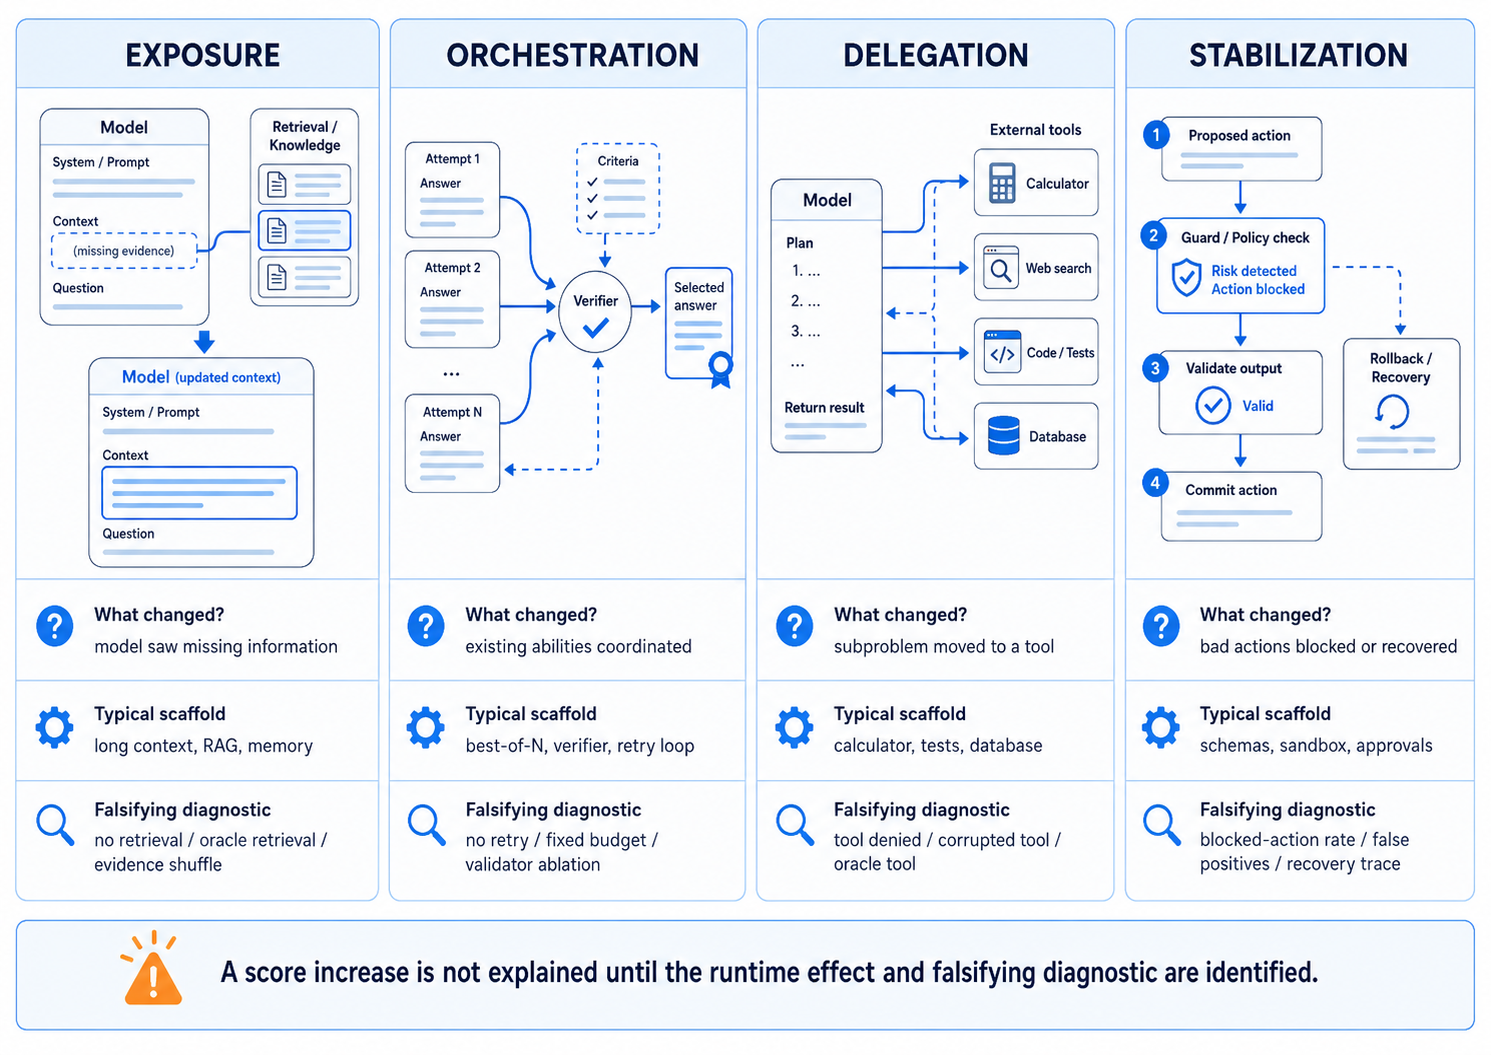
\includegraphics[width=0.96\textwidth]{figures/ch22/fig_four_effects_runtime_systems.png}
\caption{\textbf{Four effects of runtime systems.} The question is not only whether the system score improved. It is which runtime effect explains the improvement and which diagnostic would make that explanation less plausible.}
\label{fig:ch22-four-effects}
\end{figure}

\subsection{Efficiency as the Cross-Cutting Fifth Axis}

Exposure, orchestration, delegation, and stabilization explain how runtime scaffolds change behavior. Efficiency explains whether that behavior can be delivered under realistic latency, memory, throughput, and cost constraints. Some system improvements do not raise answer quality at all. They hold quality fixed while reducing cost per success, lowering latency, fitting more requests into memory, or making a larger context window affordable.

This is how Chapter~\ref{ch:serving-quantization-cost} fits into the Part~IV audit. Quantization, continuous batching, PagedAttention, speculative decoding, KV-cache optimization, and prefix caching are not always new reasoning mechanisms. They change what system behavior is affordable. A workflow that is too slow or expensive to run is not the same system once serving improvements make it practical.

Every runtime effect should therefore be evaluated on the cost, latency, memory, and throughput axes. A better exposure system may retrieve more evidence, but the audit asks whether that evidence can be packed and served cheaply. A better orchestration system may try more candidates, but the audit asks whether the extra calls are worth the task value. A better delegation system may call tools, but the audit asks whether tool latency and failure handling fit the operating setting. Efficiency is not a replacement for the four effects; it is the constraint that determines whether they can be deployed.

\subsection{Exposure: The System Shows the Model Missing Information}

Exposure means the system improves because it makes relevant information visible. Chapter~\ref{ch:long-context-retrieval-memory} was mainly about exposure. Long context, retrieval, reranking, memory, cached context, citation snippets, and context compression all try to answer the same question:

\begin{quote}
Did the model see the right evidence in a form it could use?
\end{quote}

A clean exposure success story looks like this: the closed-book model fails, oracle evidence makes the model answer correctly, and the retriever finds the same evidence often enough that the end-to-end RAG system improves. A weak exposure story looks different: the system retrieves more text, but the relevant paragraph is absent, buried, stale, or cited without supporting the claim.

The diagnostics follow directly from the mechanism. Remove retrieval. Give oracle retrieval. Shuffle evidence order. Insert distractors. Audit citations at the claim level. Compare retrieval recall with answer faithfulness. These tests do not ask whether RAG is good in general. They ask whether this system's gain came from exposure.

\subsection{Orchestration: The System Coordinates Existing Abilities}

Orchestration means the system improves by arranging attempts, validators, steps, roles, or workflow branches. Chapter~\ref{ch:inference-time-scaling} studied orchestration through inference-time compute: best-of-$N$, self-consistency, verifier reranking, and search. Chapter~\ref{ch:tool-use-agent-loops} studied orchestration through workflows and agent loops.

The core question is:

\begin{quote}
Did the system improve because it coordinated existing abilities more reliably?
\end{quote}

A clean orchestration story might say: a single call often misses the solution, but multiple samples produce a correct candidate and a verifier selects it. A planner-executor workflow may improve because planning, acting, validation, and final synthesis are separated. A retry loop may help because each retry changes the query, context, tool, timeout, or validation condition.

The failure mode is motion without progress. Reflection can become rationalization. Retrying can become repeated guessing. A workflow can overfit to the benchmark format. A high score may come from spending many more calls, not from a more reliable per-attempt policy. The right diagnostics are no-retry ablations, fixed-sample-budget comparisons, validator ablations, trace replay, and cost-per-success curves.

\subsection{Delegation: The System Outsources Subproblems}

Delegation means the runtime hands part of the task to an external tool, environment, or specialized subsystem. This is the core value of tool use. A calculator computes arithmetic. A search engine finds web pages. A database executes SQL. A compiler checks syntax. A unit test suite validates behavior. A symbolic solver handles algebra. A browser manipulates a web environment.

Delegation is not cheating. Real intelligence uses tools. But attribution must be honest.

\begin{quote}
Did the system improve because the model became more capable, or because the runtime outsourced the hard part?
\end{quote}

A calculator agent that solves arithmetic may not show that the model learned arithmetic. A coding agent that passes tests may not show that the model understood the entire repository in one pass. A database agent that answers a factual query may not show parametric memory; it may show good SQL construction plus database execution.

The diagnostics isolate the tool boundary. Compare model-only, tool-denied, tool-only where possible, oracle tool output, and corrupted tool output. Measure planning quality separately from tool execution. If the model chooses the wrong tool or ignores a correct tool result, the problem is not the tool's raw capability.

\subsection{Stabilization: The System Prevents, Catches, or Recovers from Failures}

Stabilization means the runtime improves reliability or safety by constraining actions, validating outputs, logging traces, escalating to humans, or recovering from typed failures. Chapter~\ref{ch:serving-quantization-cost} introduced reliability under production constraints. Chapter~\ref{ch:tool-use-agent-loops} made stabilization concrete through schemas, permissions, sandboxes, rollback, approval policies, budget controls, and trace logging.

The key question is:

\begin{quote}
Did the system improve because it produced better actions, or because it blocked worse ones?
\end{quote}

Both are useful. A system that blocks unsafe database writes is better than one that executes them. A stabilizing system may lower raw task success by refusing unsafe or unsupported actions. That is not necessarily regression; it changes the objective from maximum completion to bounded completion. But the score should reveal that stabilization happened. Otherwise a benchmark may report only final success while hiding unsafe attempts, over-refusals, blocked actions, or human escalations.

Useful stabilization metrics include blocked-action rate, unsafe-action attempt rate, false-positive guardrail rate, human escalation rate, recoverable versus unrecoverable failures, and safety-cost tradeoff curves.

\begin{quickrecap}
\textbf{Quick Recap.}
\begin{itemize}[nosep,leftmargin=1.5em]
  \item Exposure improves systems by showing the model missing evidence.
  \item Orchestration improves systems by coordinating attempts, validators, retries, and workflow steps.
  \item Delegation improves systems by moving subproblems to external tools or environments.
  \item Stabilization improves systems by blocking, validating, bounding, or recovering from failures.
  \item Efficiency determines whether these effects can be delivered under realistic cost, latency, memory, and throughput constraints.
\end{itemize}
\textit{Next: a system can succeed without proving that the base model itself became more capable.}
\end{quickrecap}


%----------------------------------------------------------------------
\section{System Success Is Not Model Capability}
\label{sec:ch22-system-vs-model}

Users experience systems. They do not experience isolated neural networks. If a deployed assistant answers correctly because it retrieved the right evidence, called the right tool, and validated the result, the user received real value. The system was intelligent in the practical sense that matters to the user.

Research claims require a second step: attribution. We must distinguish what the model can do from what the runtime made possible.

\begin{center}
\begin{tabularx}{\textwidth}{@{}lX@{}}
\toprule
\textbf{Concept} & \textbf{Meaning} \\
\midrule
Model capability & What the model can do inside one or more model calls, without the scaffold under study. \\
System success & What the full runtime accomplishes using context, tools, retries, validators, workflows, and constraints. \\
User-facing intelligence & What the user experiences from the complete system. \\
Attributed capability & The component-level explanation of what caused the observed success. \\
\bottomrule
\end{tabularx}
\end{center}

\subsection{Common Misattributions}

Misattribution is easy because the final answer hides the path that produced it. Five examples recur throughout model-system work:

\begin{itemize}[leftmargin=1.5em]
  \item A RAG system answering correctly does not mean the model knew the fact. It may mean the system exposed the fact.
  \item A calculator agent computing correctly does not mean the model learned arithmetic. It may mean tool delegation worked.
  \item A coding agent passing tests does not mean the model understood the whole repository in one call. It may mean executable validation and retries found a patch.
  \item A best-of-$N$ system solving a problem does not mean single-sample reliability improved. It may mean search found one good sample.
  \item A tool workflow completing a task does not mean a fully autonomous agent would complete it. It may mean the workflow encoded the right control structure.
\end{itemize}

This is not anti-system. It is pro-attribution. A strong runtime is a real engineering achievement. But a system score should not be casually converted into a claim about model-internal capability.

\subsection{User-Facing and Scientific Questions}

Two questions can both be legitimate:

\begin{enumerate}[nosep]
  \item \textbf{Product question}: did the user get the task solved reliably, safely, and affordably?
  \item \textbf{Scientific question}: which component made the task solvable, and would the gain survive if that component changed?
\end{enumerate}

Chapter~\ref{ch:frontiers} made a similar distinction for post-training. A post-trained model may improve pass@1 by moving probability mass toward trajectories the base model could already sample. That is valuable for users, but it changes what the training method is credited with. Runtime systems create the same attribution problem at the system level.

\begin{tcolorbox}[colback=gray!8, colframe=gray!40, title=\textbf{Echo: From Ch17 to Ch22}]
Chapter~\ref{ch:frontiers} asked whether post-training sharpens, composes, or discovers behavior. This chapter asks whether runtime systems expose information, orchestrate attempts, delegate subproblems, or stabilize behavior. In both cases, the goal is not to diminish the method. The goal is to describe what changed accurately.
\end{tcolorbox}

\noindent\fbox{\parbox{\dimexpr\textwidth-2\fboxsep-2\fboxrule\relax}{%
\textbf{Pause and verify.}\quad A RAG system improves accuracy from 45\% to 78\%. With oracle retrieval, the same model reaches 90\%. With retrieved evidence removed, it returns to 46\%. What is the most likely improvement story? The gain is mainly exposure: the model can use correct evidence when shown, and the system's remaining gap is retrieval quality or evidence packing, not base-model knowledge.
}}

\begin{quickrecap}
\textbf{Quick Recap.}
\begin{itemize}[nosep,leftmargin=1.5em]
  \item System success is real user-facing intelligence, but it is not automatically model capability.
  \item Research claims must attribute success to model behavior, context, tools, workflows, validation, or constraints.
  \item The same score can support different explanations unless traces, ablations, and oracle tests separate the components.
\end{itemize}
\textit{Next: the component attribution ladder turns attribution into a concrete diagnostic protocol.}
\end{quickrecap}


%----------------------------------------------------------------------
\section{Component Attribution Ladder}
\label{sec:ch22-attribution-ladder}

The main diagnostic of this chapter is the component attribution ladder. It asks:

\begin{quote}
If the full system succeeds, which component was necessary?
\end{quote}

The ladder is a sequence of controlled variants. Each rung adds one capability or replaces a component with an oracle. The purpose is not to find the best demo. The purpose is to explain the gain.

\begin{figure}[t]
\centering
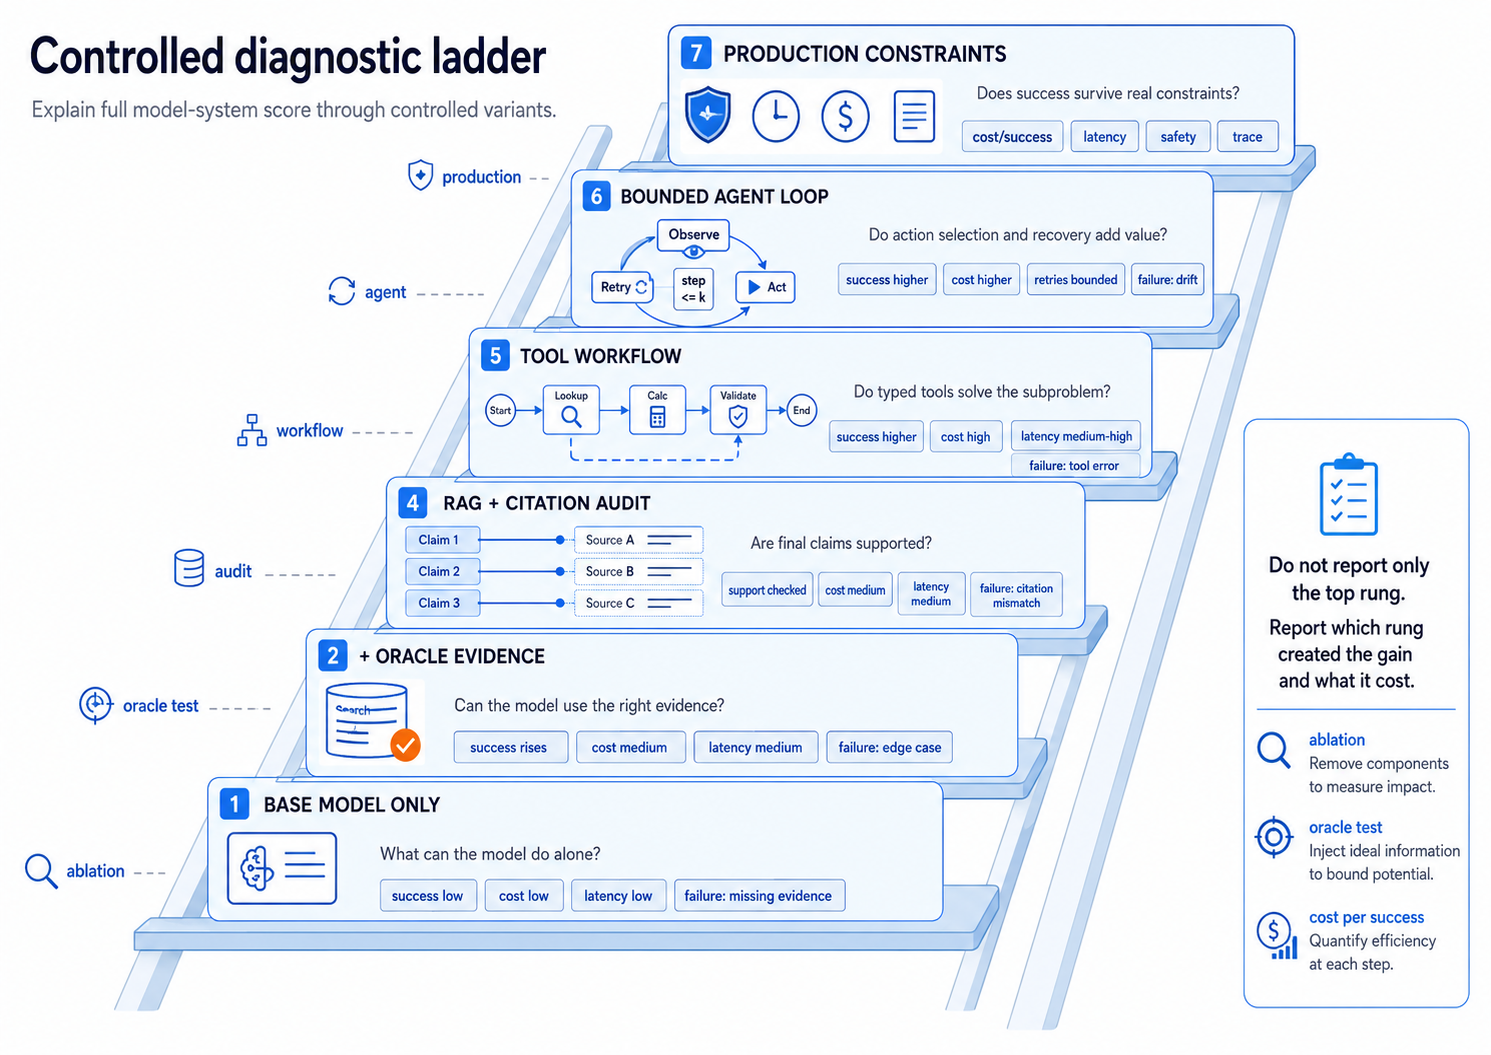
\includegraphics[width=0.96\textwidth]{figures/ch22/fig_component_attribution_ladder.png}
\caption{\textbf{Component attribution ladder.} A full-system score is explained by comparing controlled variants, not by inspecting the final answer alone. Oracle rungs distinguish model limitations from retrieval, tool, and workflow limitations.}
\label{fig:ch22-attribution-ladder}
\end{figure}

\subsection{A Worked Example}

Suppose the task is a small software repair benchmark item: resolve a GitHub issue that requires reading three files, editing one function, and passing four tests. The full agent loop succeeds. The attribution ladder might look like this:

\begin{center}
\small
\begin{tabularx}{\textwidth}{@{}lrrrrX@{}}
\toprule
\textbf{Variant} & \textbf{Tests passed} & \textbf{Calls} & \textbf{Latency} & \textbf{Cost/success} & \textbf{Main failure layer} \\
\midrule
Base model only & 0/4 & 1 & low & low but failed & hallucinates file path \\
+ oracle files & 3/4 & 1 & medium & medium & misses edge-case behavior \\
+ retrieved files & 2/4 & 2 & medium & medium & retrieval misses one file \\
+ tool workflow & 4/4 & 4 & high & high & none on this task \\
+ bounded agent loop & 4/4 & 7 & higher & higher & extra retry after weak observation \\
+ production constraints & 4/4 & 7 & bounded & acceptable & succeeds within budget \\
\bottomrule
\end{tabularx}
\end{center}

The full system succeeded, but the table changes the interpretation. Oracle files pass three of four tests, confirming that the model can use relevant evidence while revealing a residual model-level gap on an edge case. Retrieved files underperform oracle files, so file discovery is also a bottleneck. Tool execution finishes the task by making validation executable. The agent loop does not improve this particular task over the tool workflow; it adds cost. On harder tasks the loop may help, but this trace does not prove that it did.

This is the point of the ladder: it converts a single success into an attribution profile.

\subsection{Ablations, Oracles, and Scaffolding Curves}

Three families of tests appear throughout the ladder:

\begin{description}[leftmargin=1.5em]
  \item[Ablations.] Remove a component and measure what breaks: no retrieval, no memory, no tool, no retry, no verifier, no guardrail.
  \item[Oracles.] Replace a component with an idealized version: oracle evidence, oracle tool output, oracle route, oracle validator.
  \item[Scaffolding curves.] Measure success as a function of runtime budget: number of samples, model calls, tool calls, retries, latency, or dollars.
\end{description}

Ablations show necessity. Oracles show headroom. Scaffolding curves show whether the system bought success by spending more. Chapter~\ref{ch:serving-quantization-cost} introduced cost per useful task. Here the same idea becomes cost per successful system outcome:

\[
\text{cost per success} = \frac{\text{total runtime cost}}{\text{number of successful tasks}}.
\]

If a system doubles accuracy while increasing cost tenfold, it may still be useful for high-value tasks. But the improvement story must say that reliability was purchased with runtime spend. Cost per success is not minimized in isolation. The right operating point depends on task value, failure cost, latency requirements, and the cost of human review. That is different from a system that improves both success and cost per success.

Agent systems also require repeatability, not only a best trajectory. Sampling randomness, tool instability, web state changes, different retry paths, nondeterministic execution, and judge variance can make the same system succeed once and fail later. A system result should report variance across runs when repeated trials are feasible. For agent systems, repeatability is part of reliability.

\subsection{Project 4 Report Template}

\begin{tcolorbox}[colback=orange!5, colframe=orange!60, title=\textbf{For Project 4: Report an Attribution Profile}]
For your final Project~4 report, compare at least four variants:
\begin{enumerate}[nosep]
  \item plain assistant;
  \item RAG assistant;
  \item tool workflow;
  \item bounded agent loop.
\end{enumerate}
For each variant, report task success, cost per attempt, cost per success, latency, model calls, tool calls, retries, citation support, tool success, trace quality, safety incidents or blocked actions, run-to-run variance, number of repeated trials per task, best-run versus average-run performance, failure consistency, and first broken failure layer. Do not only show the best demo. Explain which component made the system better and what it cost.
\end{tcolorbox}

\begin{quickrecap}
\textbf{Quick Recap.}
\begin{itemize}[nosep,leftmargin=1.5em]
  \item The component attribution ladder compares controlled variants from base model to full production system.
  \item Ablations test necessity; oracles test headroom; scaffolding curves test how success scales with runtime budget.
  \item Cost per success is often more informative than raw accuracy for model systems, but the right operating point depends on task value and failure cost.
  \item Agent results should report run-to-run variance when repeated trials are feasible.
\end{itemize}
\textit{Next: when a system fails, the same discipline localizes the first broken layer.}
\end{quickrecap}


%----------------------------------------------------------------------
\section{Find the First Broken Layer}
\label{sec:ch22-first-broken-layer}

When a model system fails, the least useful diagnosis is ``the model failed.'' Sometimes that is true. Often it is too vague. A system may fail because retrieval missed the key document, a summary distorted evidence, a tool call used invalid arguments, a workflow routed to the wrong branch, the scratchpad became stale, the validator was weak, or the budget stopped the loop early.

The practical diagnostic is:

\begin{quote}
Localize the first broken layer.
\end{quote}

\begin{figure}[t]
\centering
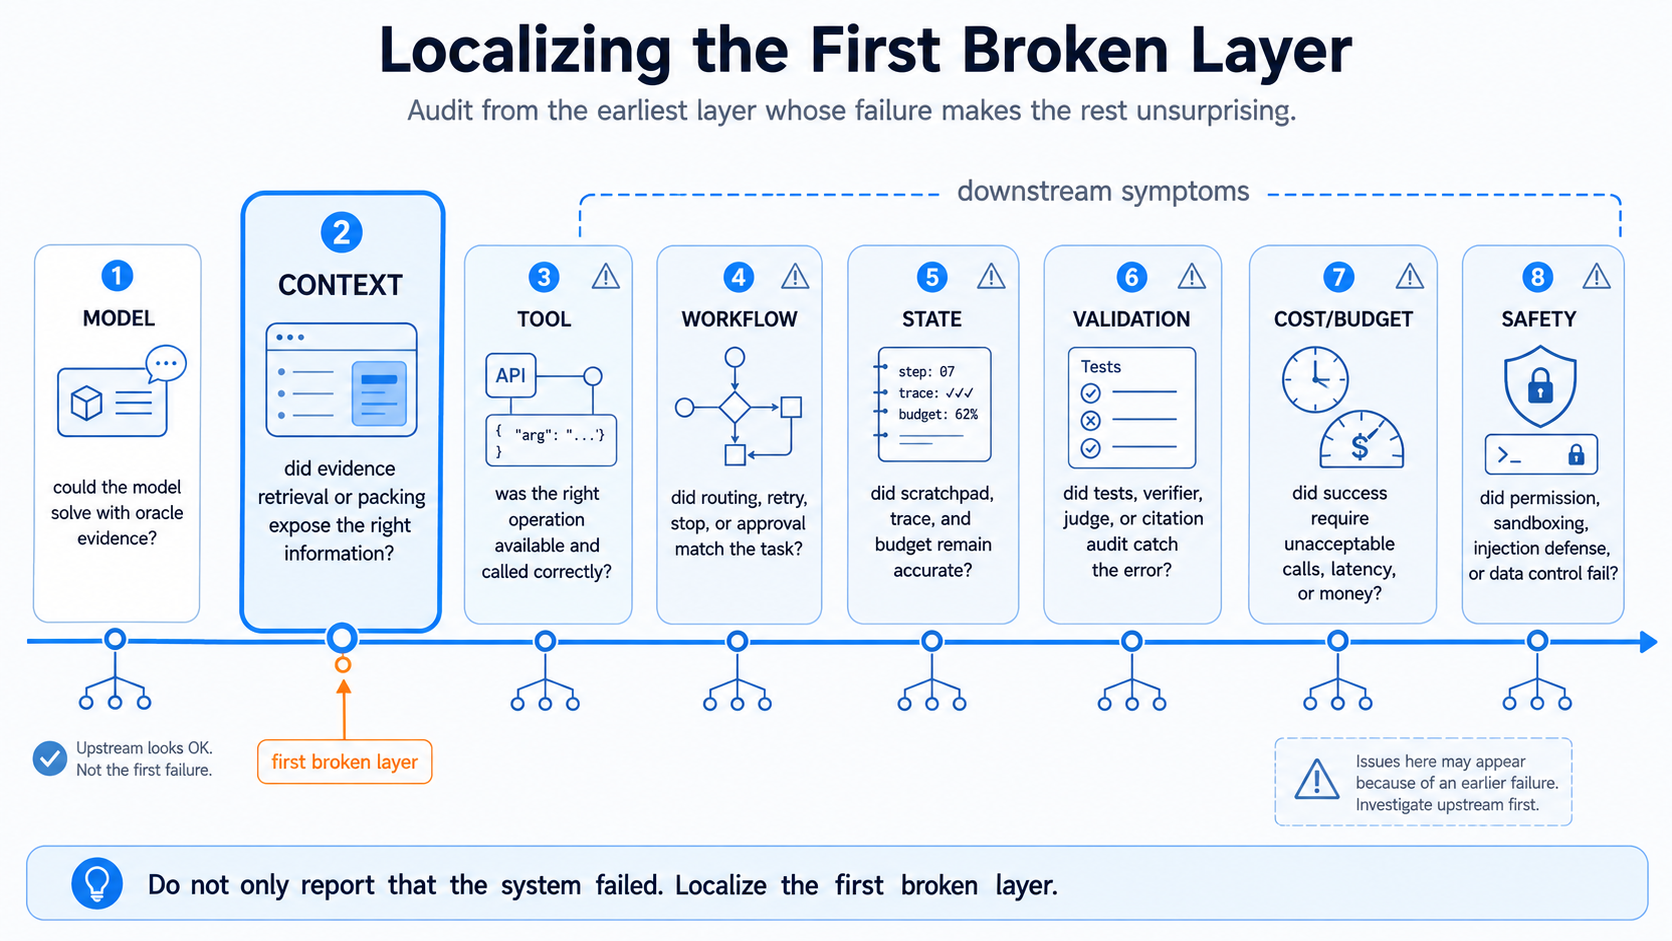
\includegraphics[width=0.96\textwidth]{figures/ch22/fig_failure_attribution_tree.png}
\caption{\textbf{Failure attribution tree.} The goal is not to list every possible bug. It is to find the first layer whose failure made later failures unsurprising.}
\label{fig:ch22-failure-tree}
\end{figure}

\subsection{A Short Procedure}

A compact failure review can follow this order:

\begin{enumerate}[leftmargin=1.5em]
  \item \textbf{Check the model floor.} With oracle evidence and no tools, can the model produce the right answer or plan?
  \item \textbf{Check exposure.} Did the system retrieve, remember, or pack the evidence required for success?
  \item \textbf{Check action.} Did the workflow choose the right tool or branch, and were arguments valid?
  \item \textbf{Check observation use.} Did the model interpret tool output, test failures, or citations correctly?
  \item \textbf{Check state.} Did the runtime update scratchpad, trace, budget, and pending tasks correctly?
  \item \textbf{Check validation.} Did the validator catch wrong outputs, unsupported claims, unsafe actions, or failed tests?
  \item \textbf{Check budget and safety.} Did the system stop for a principled reason, and were side effects bounded?
\end{enumerate}

This procedure deliberately crosses the boundaries of earlier chapters. Ch20 taught context diagnostics. Ch21 taught trace diagnostics. Ch22 asks which layer broke first in the full stack.

\subsection{A Worked Failure}

Consider a research assistant that answers a factual question with a citation. The final answer is wrong. Trace review shows that the model cited a source that discusses a related topic but does not support the claim.

The first broken layer may not be the final-answer model. If oracle retrieval gives the model the right paragraph and it answers correctly, the model floor is adequate. If the retriever never surfaced the correct paragraph, the first broken layer is context. If the retriever surfaced it but the packer placed it below many distractors, the failure is evidence packing. If the correct paragraph was visible and the model still cited the wrong source, the failure is reading or citation attribution. If the citation audit would have caught the mismatch but was disabled for latency, the failure is validation or budget policy.

The label matters because the fix differs. A model failure suggests a better model or task decomposition. A retrieval failure suggests indexing, query expansion, reranking, or corpus coverage. A validation failure suggests claim-level citation audit. A budget failure suggests an explicit cost-reliability tradeoff.

\noindent\fbox{\parbox{\dimexpr\textwidth-2\fboxsep-2\fboxrule\relax}{%
\textbf{Pause and verify.}\quad A tool agent calls the right database API, gets the correct row, but then writes a final answer using an older value from its scratchpad. Which layer broke first? The tool layer worked. The failure is state or observation use: the runtime/model did not update the task-local state from the fresh observation before final synthesis.
}}

\begin{quickrecap}
\textbf{Quick Recap.}
\begin{itemize}[nosep,leftmargin=1.5em]
  \item System failures should be localized to the first broken layer, not blamed generically on the model.
  \item Ch22 unifies Ch20 context diagnostics and Ch21 trace diagnostics into cross-layer failure attribution.
  \item The same final error can require different fixes depending on whether the first broken layer is model, context, tool, workflow, state, validation, cost, or safety.
\end{itemize}
\textit{Next: even when benchmarks improve, runtime scaffolds can overfit the benchmark interface.}
\end{quickrecap}


%----------------------------------------------------------------------
\section{Scaffold-Level Goodhart}
\label{sec:ch22-scaffold-goodhart}

Chapter~\ref{ch:evaluation} introduced Goodhart's Law for model evaluation: when a metric becomes a target, it can stop measuring what we care about. Runtime systems create a more specific version:

\begin{quote}
The model weights may stay fixed while the scaffold overfits the benchmark.
\end{quote}

This is scaffold-level Goodhart. It happens when prompt templates, retrieval policies, retry budgets, workflow graphs, tool choices, validators, or benchmark-specific heuristics are tuned until the score rises, while transfer to fresh tasks does not improve.

\subsection{How Runtime Scaffolds Overfit}

System scaffolds have many degrees of freedom:

\begin{itemize}[nosep,leftmargin=1.5em]
  \item a benchmark-specific prompt template;
  \item a file-discovery heuristic tailored to one repository layout;
  \item an unreported retry budget;
  \item a verifier that rewards benchmark formatting more than correctness;
  \item a tool that silently exposes hidden benchmark information;
  \item a workflow branch that assumes the benchmark's task grammar;
  \item a guardrail that refuses difficult cases and reports only accepted tasks.
\end{itemize}

None of these require changing the model. The system score can rise because engineers learned the benchmark interface. That can be useful engineering, but it is weak evidence of general model-system progress.

For example, a coding-agent scaffold might learn a SWE-bench-specific file-discovery rule: search for the issue's error string, open the first matching test, then edit the nearest implementation file. This can raise the benchmark score on repositories that follow that layout. If the same scaffold fails on projects with different test organization or issue phrasing, the gain was not a general improvement in code understanding. The model weights did not change; the runtime learned a narrow benchmark interface.

\subsection{Benchmark Pressure Shapes Scaffolds}

Benchmarks do not merely measure systems. They shape the runtime scaffolds people build. Static question-answering benchmarks reward single-answer correctness. RAG benchmarks reward evidence exposure, retrieval recall, and citation faithfulness. Web and tool benchmarks reward interaction reliability, state tracking, and recovery after tool failures. Coding benchmarks reward file discovery, executable validation, and patch iteration. Customer-service benchmarks such as \(\tau\)-bench reward repeatable policy following across tool calls, database state, and user interaction.

As benchmarks change, scaffolds change with them. That is healthy when the benchmark pressure moves systems toward real deployment requirements. It becomes Goodhart when the scaffold learns the benchmark interface more than the task. The audit question is whether the design pressure produced a general capability pattern or a narrow route through the benchmark.

\subsection{Real Progress Versus Scaffolding Artifact}

\begin{center}
\begin{tabularx}{\textwidth}{@{}XX@{}}
\toprule
\textbf{Real system progress} & \textbf{Scaffolding artifact} \\
\midrule
Improvement survives fresh tasks, perturbations, and new task templates. & Improvement disappears when task wording, interface, or corpus changes. \\
Failure modes shrink and traces show genuine recovery. & Failures are hidden by retries, refusals, filters, or cherry-picked runs. \\
Cost per success improves or stays justified for the task value. & Accuracy rises only by spending many more calls or hidden tool cost. \\
Tool use remains robust when tools fail, time out, or return noisy results. & Tool use assumes benchmark-specific outputs or perfect tool behavior. \\
Validation catches unsupported claims and unsafe actions. & Validators reward formatting, superficial agreement, or test gaming. \\
\bottomrule
\end{tabularx}
\end{center}

The central question is:

\begin{quote}
Has the system learned a general task strategy, or has the scaffold learned the benchmark interface?
\end{quote}

\subsection{What to Report}

Responsible system reporting should include the details that let readers distinguish real progress from scaffold artifacts:

\begin{itemize}[nosep,leftmargin=1.5em]
  \item number of model calls, retries, tool calls, and human interventions;
  \item token, latency, and dollar cost per attempt and per success;
  \item tool access, tool failure handling, and whether tools see hidden state;
  \item validation rules, test leakage risks, and judge prompts if applicable;
  \item ablation results for retrieval, tools, retries, validators, and guardrails;
  \item repeated-trial statistics: variance across runs, best run versus average run, and failure consistency;
  \item performance under fresh tasks, perturbations, or changed interfaces.
\end{itemize}

The goal is not to make every paper or project report enormous. The goal is to prevent a single score from hiding the runtime machinery that produced it.

\begin{quickrecap}
\textbf{Quick Recap.}
\begin{itemize}[nosep,leftmargin=1.5em]
  \item Scaffold-level Goodhart occurs when the runtime scaffold overfits the benchmark while the model weights may not change.
  \item System scores can be inflated by benchmark-specific prompts, workflows, retries, tools, validators, or hidden costs.
  \item Fresh tasks, perturbations, repeatability, cost-per-success, and trace transparency help distinguish real progress from scaffold artifacts.
\end{itemize}
\textit{Next: the same audit questions define the open problems for model systems.}
\end{quickrecap}


%----------------------------------------------------------------------
\section{Open Problems for Model Systems}
\label{sec:ch22-open-problems}

Part~IV did not end with a solved engineering stack. It ended with a research agenda. The components now exist: inference-time compute, serving infrastructure, long context, retrieval, memory, tools, workflows, and agent loops. The frontier is knowing how to make them reliable, attributable, affordable, and transferable.

\subsection{Why These Are Research Problems}

These problems are not only product polish. They affect what claims the field can make.

If component attribution is weak, a system score cannot tell us what improved. If cost-reliability tradeoffs are hidden, expensive scaffolds can look like capability progress. If context faithfulness is weak, RAG systems may produce supported-looking hallucinations. If trace reliability is weak, agent loops can look purposeful while drifting. If scaffolds do not generalize, benchmark progress will not predict deployment performance. If tool safety and oversight remain ad hoc, useful delegation will be limited by side-effect risk.

\begin{center}
\small
\begin{tabularx}{\textwidth}{@{}p{0.20\textwidth}p{0.16\textwidth}p{0.27\textwidth}X@{}}
\toprule
\textbf{Open problem} & \textbf{Where it came from} & \textbf{Core question} & \textbf{What would count as progress?} \\
\midrule
Component attribution & Ch18--21 & Which component caused the gain? & Ablations and oracle tests explain most score changes. \\
Cost-reliability frontier & Ch19 & Is higher success worth the runtime spend? & Cost per success and latency are reported with quality and task value. \\
Context faithfulness & Ch20 & Did the answer use the cited evidence? & Claim-level support audits become routine. \\
Trace reliability & Ch21 & Did the loop recover or drift? & Trace diagnostics localize the first broken layer. \\
Scaffold generalization & Ch21--22 & Does the scaffold transfer beyond benchmark format? & Gains survive task perturbations, repeated runs, and fresh interfaces. \\
Benchmark decay & Ch10/22 & Has the benchmark saturated, leaked, or been gamed? & Fresh hidden tasks and contamination audits exist. \\
Tool safety & Ch21 & Can tools be used without unsafe side effects? & Sandbox, permission, injection, and escalation tests pass. \\
\bottomrule
\end{tabularx}
\end{center}

\begin{figure}[t]
\centering
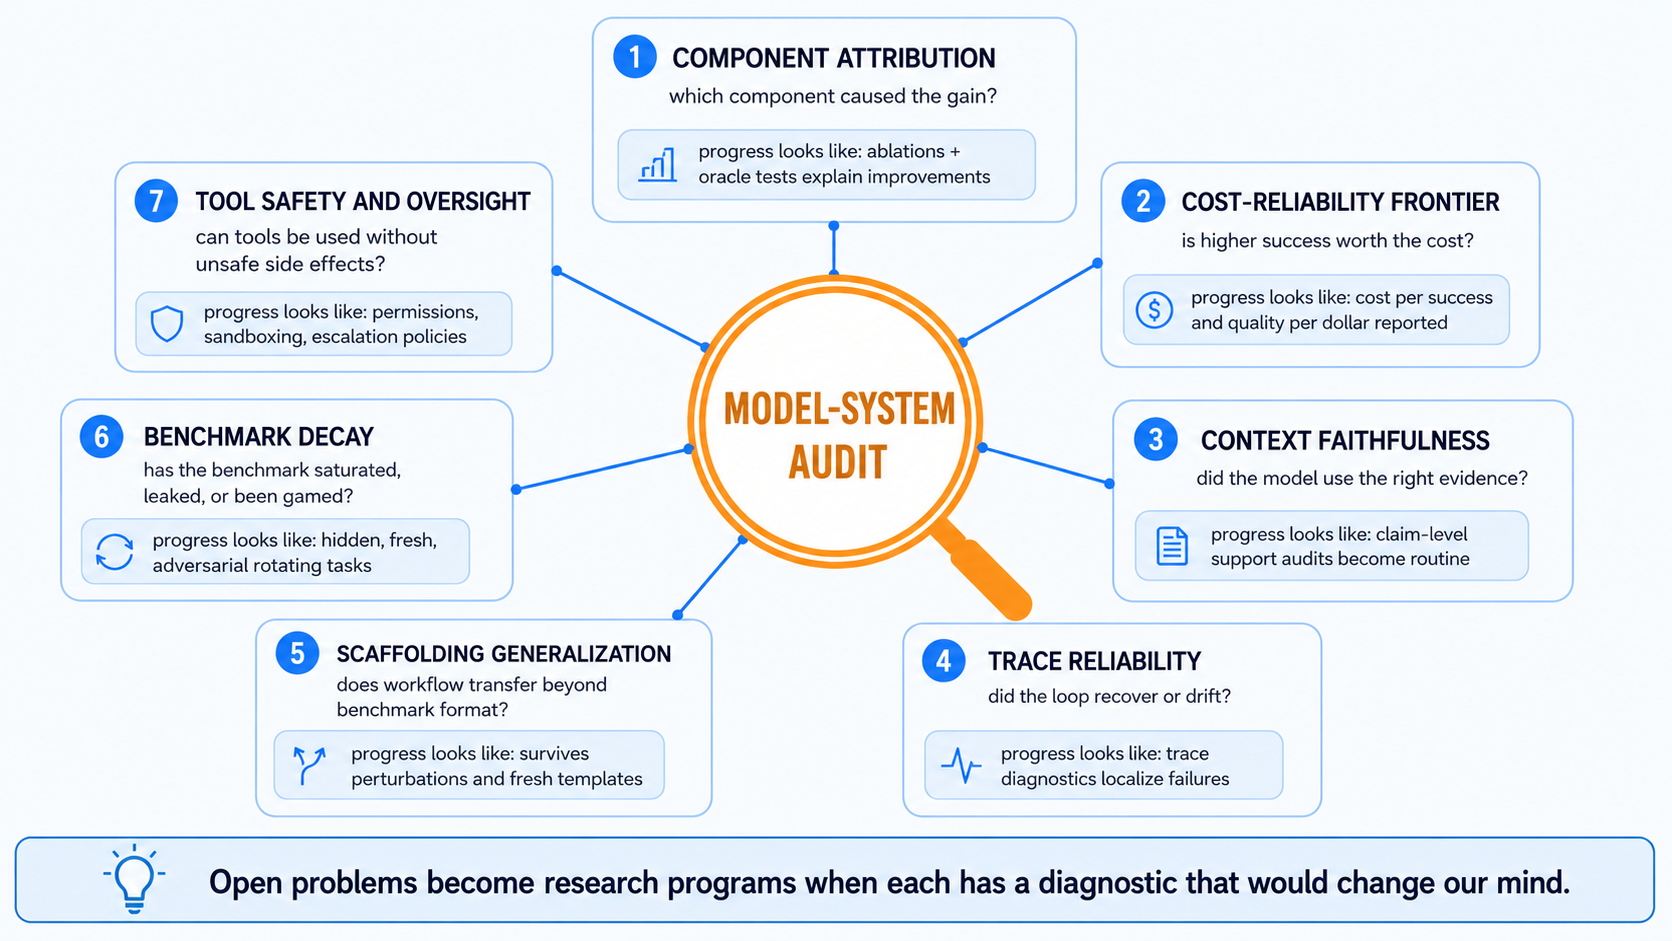
\includegraphics[width=0.96\textwidth]{figures/ch22/fig_open_problems_audit_targets.png}
\caption{\textbf{Open problems as audit targets.} Each open problem pairs a system frontier with a diagnostic standard.}
\label{fig:ch22-open-problems}
\end{figure}

\subsection{The Research Habit}

The durable habit is to convert every system failure into an audit question:

\begin{itemize}[nosep,leftmargin=1.5em]
  \item Which component was responsible?
  \item What would an oracle version of that component achieve?
  \item What ablation would make the claimed mechanism disappear?
  \item What did the scaffold cost?
  \item What new failure did it introduce?
  \item Would the gain survive a fresh task distribution?
\end{itemize}

That habit will matter even more in later parts of the book. Multimodal systems add visual evidence and cross-modal alignment. World-model systems add latent dynamics, prediction, planning, and action in simulated or physical environments. The audit discipline remains the same: locate the source of success and the first broken layer.

\begin{quickrecap}
\textbf{Quick Recap.}
\begin{itemize}[nosep,leftmargin=1.5em]
  \item The main open problems for model systems are attribution, cost-reliability, context faithfulness, trace reliability, scaffold generalization, benchmark decay, and tool safety.
  \item Each open problem should be paired with a concrete criterion for progress.
  \item The audit habit transfers to multimodal and world-model systems.
\end{itemize}
\textit{Next: we close Part~IV by summarizing what the runtime stack added to foundation models.}
\end{quickrecap}


%----------------------------------------------------------------------
\section{Part IV Closing Reflection}
\label{sec:ch22-closing-reflection}

Part~IV began with a simple observation: a foundation model at inference time is not just a frozen function from prompt to answer. It is often embedded in a runtime system. That runtime can spend more compute, serve requests efficiently, retrieve evidence, remember state, call tools, execute workflows, validate outputs, recover from errors, and expose traces.

This changes what we mean by capability. The base model matters enormously. But user-facing intelligence often comes from the system around it. A model that cannot answer closed book may answer with retrieval. A model that cannot guarantee arithmetic may call a calculator. A model that cannot know whether a patch works may run tests. A model that may attempt an unsafe action may be bounded by permissions, sandboxing, and human approval.

The Part~IV lesson is not that scaffolding replaces models. It is that models and scaffolds must be evaluated together and attributed separately.

\begin{quote}
Part~IV taught how to turn a model into a system. The audit habit is to ask whether the system's success came from better information, better orchestration, external delegation, safer stabilization, or merely a more expensive way to hide the same failure.
\end{quote}

\begin{quickrecap}
\textbf{Quick Recap.}
\begin{itemize}[nosep,leftmargin=1.5em]
  \item Runtime systems turn frozen model calls into user-facing capabilities.
  \item The same system score can reflect exposure, orchestration, delegation, stabilization, or benchmark-specific scaffolding.
  \item The closing habit of Part~IV is attribution: explain the source, cost, and failure modes of every system gain.
\end{itemize}
\textit{Next: Part~V adds visual evidence and cross-modal grounding to the same system questions.}
\end{quickrecap}


%----------------------------------------------------------------------
\section*{Summary}
\label{sec:ch22-summary}

This chapter established Ch22 as the Part~IV closing audit chapter. Chapters~\ref{ch:inference-time-scaling}--\ref{ch:tool-use-agent-loops} taught runtime scaffolds: inference-time compute, serving infrastructure, long context, retrieval, memory, tools, workflows, and agent loops. Ch22 asked what those scaffolds actually changed.

\paragraph{The model-system audit lesson.} A model system is not understood from its final score alone. The score may come from exposure, orchestration, delegation, stabilization, or scaffold-specific overfitting. The audit task is to identify which component caused the gain, which bottleneck it removed, what cost it introduced, and which diagnostic would falsify the story.

\paragraph{One sentence.} Users experience systems, but research claims must attribute system success to model behavior, context, tools, workflows, validation, constraints, cost, and traces.

\paragraph{What comes next.} Part~V moves from text-only systems to multimodal foundation models. Visual encoders, image tokens, cross-modal alignment, and grounded reasoning will add new kinds of evidence and new failure layers. The audit discipline from this chapter carries forward: ask what the system saw, what it did, what it delegated, what it validated, and where it first broke.

\begin{takeaways}
\begin{itemize}
  \item Ch22 is not a benchmark catalog; it is an epistemic audit of Part~IV runtime scaffolds.
  \item Runtime systems improve model behavior through exposure, orchestration, delegation, and stabilization.
  \item System success is user-facing and real, but it should not be confused with model-internal capability.
  \item The component attribution ladder uses ablations, oracle components, and cost-normalized comparisons to explain gains.
  \item Failure attribution should localize the first broken layer across model, context, tool, workflow, state, validation, cost, and safety.
  \item Scaffold-level Goodhart occurs when prompts, workflows, retries, tools, or validators overfit benchmark interfaces.
  \item Open problems for model systems include attribution, cost-reliability, context faithfulness, trace reliability, scaffold generalization, benchmark decay, and tool safety.
\end{itemize}
\end{takeaways}

\section*{Key Equations and Concepts}

\begin{center}
\begin{tabularx}{\textwidth}{@{}lX@{}}
\toprule
\textbf{Expression} & \textbf{Interpretation} \\
\midrule
$S = M + X$ & A model system combines a base model $M$ with runtime scaffold $X$. This is conceptual, not a literal additive model. \\
$A(S,T) - A(M,T)$ & The observed system gain that requires attribution. \\
$\Delta_X$ & Improvement associated with component $X$ under a specified ablation or oracle comparison. \\
$\text{cost per success} = C / \#\text{successes}$ & Cost-normalized reliability metric for system comparisons. \\
$F = \operatorname{first\_broken\_layer}(\tau)$ & Failure review should localize the earliest layer in the trace that made later failure likely. \\
Exposure / orchestration / delegation / stabilization & Four runtime effects that explain most model-system gains. \\
\bottomrule
\end{tabularx}
\end{center}

\section*{Key Checks}

\begin{itemize}
  \item Explain why a model-system benchmark score does not measure the model alone.
  \item Classify a runtime improvement as exposure, orchestration, delegation, stabilization, or a combination.
  \item Given a RAG result, design no-retrieval, oracle-retrieval, evidence-shuffling, and citation-audit diagnostics.
  \item Given a tool-agent result, design tool-denied, corrupted-tool, oracle-tool, and trace-replay diagnostics.
  \item Build a component attribution ladder for a plain assistant, RAG assistant, tool workflow, and bounded agent loop.
  \item Interpret a cost-per-success curve and decide whether a higher score is worth the runtime spend.
  \item Given a failed trace, identify the first broken layer and propose the right class of fix.
  \item Distinguish real system progress from scaffold-level Goodhart.
\end{itemize}

\section*{Key Readings}

\begin{itemize}
  \item Liang et al., ``Holistic Evaluation of Language Models''~\cite{liang2022helm}. Read for the principle that evaluation should be multi-metric rather than a single leaderboard score.
  \item Lewis et al., ``Retrieval-Augmented Generation for Knowledge-Intensive NLP Tasks''~\cite{lewis2020rag}. Read as the canonical exposure scaffold.
  \item Yao et al., ``ReAct: Synergizing Reasoning and Acting in Language Models''~\cite{yao2023react}. Read for traceable interleaving of reasoning and action.
  \item Zheng et al., ``Judging LLM-as-a-Judge with MT-Bench and Chatbot Arena''~\cite{zheng2023judging}. Read for the usefulness and bias risks of model-based evaluation.
  \item SWE-bench and SWE-agent~\cite{jimenez2024swebench,yang2024sweagent}. Read as coding-agent case studies where executable validation changes the reliability frontier.
  \item WebArena, AgentBench, and \(\tau\)-bench~\cite{zhou2023webarena,liu2023agentbench,yao2024taubench}. Read as examples of benchmark pressure moving from demos toward interactive reliability.
\end{itemize}

\flushbottom
